\documentclass[
	main=english,
	ruledheaders=section,%Ebene bis zu der die Überschriften mit Linien abgetrennt werden
	class=book,% Basisdokumentenklasse
	thesis={type=pp},% Dokumententyp Thesis
	accentcolor=9c,% Auswahl der Akzentfarbe
	custommargins=false, %=true Ränder werden mithilfe von typearea automatisch berechnet (für jede Schriftgröße anders oder so)
	marginpar=false,% Kopfzeile und Fußzeile erstrecken sich nicht über die Randnotizspalte
	BCOR=5mm,%Bindekorrektur
	DIV=10, %gegen Whitespace
	twoside,
	parskip=half-,%Absatzkennzeichnung durch Abstand
	fontsize=11pt,%Basisschriftgröße laut Corporate Design ist mit 9pt häufig zu klein
	%	logofile=example-image, %Falls die Logo Dateien nicht vorliegen
]{tudapub}

%\geometry{reset,left=20mm, bottom=35mm, right=20mm, top=30mm}

% Englische Sprache 
\usepackage[english]{babel}
% Umlaute
\usepackage[utf8]{inputenc}

% Blockkommentare
\usepackage{comment}
% Beispiel:
% \begin{comment}
% 	Text wird nicht angezeigt
% \end{comment}

% Pakete mit Mathesymbolen und zur Beseitigung von Schwächen der Mathe-Umgebung
\usepackage{latexsym,exscale,stmaryrd,amsmath}

% Farbe
\usepackage{color}

%Bibliography and citation
\usepackage{natbib}
%\bibliographystyle{bib-sarah_english}
\bibliographystyle{thesis_sgrimm}

\usepackage{url}


% Für Einheiten
\usepackage[per-mode=symbol]{siunitx}
\sisetup{separate-uncertainty,output-decimal-marker={.},list-final-separator={\text{ and }},list-pair-separator={\text{ and }},list-separator={, },list-units=single}
\sisetup{range-phrase={\text{ to }},range-units=brackets, list-units=brackets}
\sisetup{print-zero-exponent=false, print-unity-mantissa=false}
\sisetup{detect-all}
%\sisetup{scientific-notation = engineering}

%für Reaktionsgleichungen
\usepackage{mhchem}


% Für Captions / Bildunterschriften - keine Einrückung in der zweiten Zeile mehr
\setcapindent{0pt}

%flush figures
\usepackage{placeins}
\usepackage{float}

% Zur Graphikausgabe
%Beipiel: \includegraphics[width=\textwidth]{grafik.png}
\usepackage{graphicx}

\usepackage{graphicx,import}

% Text umfließt Graphiken und Tabellen
% Beispiel:
% \begin{wrapfigure}[Zeilenanzahl]{"l" oder "r"}{breite}
%   \centering
%   \includegraphics[width=...]{grafik}
%   \caption{Beschriftung} 
%   \label{fig:grafik}
% \end{wrapfigure}
\usepackage{wrapfig}

% Mehrere Abbildungen nebeneinander
% Beispiel:
% \begin{figure}[htb]
%   \centering
%   \subfigure[Beschriftung 1\label{fig:label1}]
%   {\includegraphics[width=0.49\textwidth]{grafik1}}
%   \hfill
%   \subfigure[Beschriftung 2\label{fig:label2}]
%   {\includegraphics[width=0.49\textwidth]{grafik2}}
%   \caption{Beschriftung allgemein}
%   \label{fig:label-gesamt}
% \end{figure}
\usepackage[normalsize]{subfigure}
%normal size 


% Caption neben Abbildung
% Beispiel:
% \sidecaptionvpos{figure}{"c" oder "t" oder "b"}
% \begin{SCfigure}[rel. Breite (normalerweise = 1)][hbt]
%   \centering
%   \includegraphics[width=0.5\textwidth]{grafik.png}
%   \caption{Beschreibung}
%   \label{fig:}
% \end{SCfigure}
\usepackage{sidecap}


%Forloop 
% \foreach \n in {apples, burgers, cake}{Let's eat \n.}
\usepackage{pgffor}

% arithmetic
\usepackage{fp}

% Flowcharts
\usepackage{tikz}
\usetikzlibrary{decorations.pathreplacing}
\usetikzlibrary{shapes,arrows}
% Define tud colors
\definecolor{tudred}{RGB}{185,15,34}
\definecolor{1c}{RGB}{0,78,138}
\definecolor{2c}{RGB}{0,104,157}
\definecolor{3c}{RGB}{0,136,119}
\definecolor{4c}{RGB}{127,171,22}
\definecolor{5c}{RGB}{177,189,0}
\definecolor{6c}{RGB}{215,172,0}
\definecolor{7c}{RGB}{210,135,0}
\definecolor{8c}{RGB}{204,76,3}
\definecolor{9c}{RGB}{185,15,34}
\definecolor{10c}{RGB}{149,17,105}
\definecolor{11c}{RGB}{97,28,115}

% Define block styles
\tikzstyle{startstop} = [rectangle, rounded corners, minimum width=3cm, minimum height=1cm,text centered, draw=black, fill=red!30]
\tikzstyle{io} = [trapezium, trapezium left angle=70, trapezium right angle=110, minimum width=3cm, minimum height=1cm, text centered, draw=black, fill=2c!40]
\tikzstyle{ini} = [rectangle, minimum width=3cm, minimum height=1cm, text centered, draw=black, fill=black!10]
\tikzstyle{process} = [rectangle, minimum width=3cm, minimum height=1cm, text centered, draw=black, fill=7c!40]
\tikzstyle{dependent process} = [rectangle, minimum width=3cm, minimum height=1cm, text centered, draw=black, fill=8c!40]
\tikzstyle{information} = [rectangle, minimum width=3cm, minimum height=1cm, text centered, draw=white]
\tikzstyle{decision} = [diamond, minimum width=3cm, minimum height=1cm, text centered, draw=black, fill=4c!40]

\tikzstyle{line} = [draw, -latex']
\tikzstyle{arrow} = [->, >=latex', shorten >=1pt, thick]

\tikzstyle{fs_pc} = [rectangle, minimum width=3cm, minimum height=1cm, text centered, draw=black, fill=9c!15]
\tikzstyle{pp_pc} = [rectangle, minimum width=3cm, minimum height=1cm, text centered, draw=black, fill=2c!15]
\tikzstyle{fs} = [rectangle, minimum width=3cm, minimum height=1cm, text centered, draw=black, fill=9c!50]
\tikzstyle{pp} = [rectangle, minimum width=3cm, minimum height=1cm, text centered, draw=black, fill=2c!50]


\usetikzlibrary{calc}

\makeatletter
\newcommand{\gettikzxy}[3]{%
  \tikz@scan@one@point\pgfutil@firstofone#1\relax
  \edef#2{\the\pgf@x}%
  \edef#3{\the\pgf@y}%
}
\makeatother
% Beispiel
% \gettikzxy{(A)}{\ax}{\ay}




\usepackage[stable]{footmisc}
%\usepackage[ngerman,pdfview=FitH,pdfstartview=FitV]{hyperref}
%\usepackage[figure]{hypcap}


\usepackage{booktabs}
\usepackage{multirow}
\usepackage{longtable}
\usepackage{tabularx}
\newcolumntype{C}[1]{>{\centering\arraybackslash}m{#1}} % für vertikales und horizontales zentrieren (Funktioniert nur manchmal)

%%%%%%% CODE
\usepackage{listings}
\usepackage{color}

\definecolor{dkgreen}{rgb}{0,0.6,0}
\definecolor{gray}{rgb}{0.5,0.5,0.5}
\definecolor{mauve}{rgb}{0.58,0,0.82}

\lstset{frame=tb,
  language=IDL,
  aboveskip=3mm,
  belowskip=3mm,
  showstringspaces=false,
  columns=flexible,
  basicstyle={\small\ttfamily},
  morecomment=[l]{\#},
  numbers=none,
  numberstyle=\tiny\color{gray},
  keywordstyle=\color{blue},
  commentstyle=\color{dkgreen},
  stringstyle=\color{mauve},
  breaklines=true,
  breakatwhitespace=true,
  tabsize=3
}

%%% APPENDIX
\usepackage{pdfpages}
% include all the pages in the PDF file:
% \includepdf[pages=-]{myfile.pdf}
% 
% include just the first page of the PDF:
% \includepdf[pages={1}]{myfile.pdf}

%set default PDF version to ca. 2008 PDF v1.7
\pdfminorversion=7

% NOTES
\newcommand\myworries[1]{\textcolor{9c}{#1}}
% \renewcommand\myworries[1]{}
\usepackage{fontspec}
\newcommand\zemax[1]{{\fontspec{monospace}\selectfont{#1}}}



\begin{document} 


\Metadata{
	title=Design of an Interferometer for the Measurement of the Free Electron Density in a Laser-Generated Plasma,
	author=Sarah Grimm
}

\title{Design of an Interferometer for the Measurement of the Free Electron Density in a Laser-Generated Plasma}
\subtitle{Design eines Interferometers zur Messung der freien Elektronendichte in einem lasererzeugten Plasma}
\author[Sarah Jane Grimm]{Sarah Jane Grimm}%optionales Argument ist die Signatur,
\birthplace{Wiesbaden}%Geburtsort, bei Dissertationen zwingend notwendig
\reviewer{Prof. Dr. Markus Roth \and Haress Nazary} %Gutachter

%Diese Felder werden untereinander auf der Titelseite platziert.
%\department ist eine notwendige Angabe, siehe auch dem Abschnitt `Abweichung von den Vorgaben für die Titelseite'
\department{phys} 
\institute{Institut für Kernphysik}
\group{Laser- und Plasmaphysik \\ Prof. Dr. Markus Roth}

\date{\today}
\examdate{\today}

%	\tuprints{urn=1234,printid=12345}
%	\dedication{Für alle, die \TeX{} nutzen.}

  

\maketitle

\pagenumbering{roman}

\affidavit

\tableofcontents

\newpage

\listoffigures
  
\newpage

\pagenumbering{arabic}
  
\input{Introduction2}

\input{Experimental_Campaign}

\input{Theoretical_Framework2}

\input{System_Design}

\input{System_Assembly}

\input{Conclusion_And_Outlook}

%\input{Acknowledgements}

\newpage
\bibliography{Proposal}


\appendix
\addappheadtotoc
\renewcommand{\thechapter}{\Roman{chapter}}
\renewcommand{\thesection}{\roman{section}}

\chapter{Crystal Considerations}
\label{section: crystal}

The choice 
of crystal for the spectrometers took several 
aspects into account: 
\begin{itemize}
	\item \textbf{Lattice Spacing:} The lattice 
	spacing must lie in a range that ensures the 
	Bragg condition is fulfilled for reasonable 
	incident angles depending on the spectrometer 
	geometry and the consideration 2 outlined above. 
	\item \textbf{Diffraction Order:} Reflection 
	in the first order is preferred, as the lower 
	orders 
	typically display 
	higher reflection efficiency and cover a lower 
	energy range, corresponding to higher intensities 
	from the plasma source compared 
	to intensities at higher energies 
	\citep{monot2002high, 
	renner2019challenges}. 
	\item \textbf{Bendability:} A bent crystal 
	allows for high intensities on the detector 
	and reduces shot-to-shot fluctuations 
	\citep{levy2010double}. It could also potentially 
	offer spatial resolution. 
	\item \textbf{Intrinsic Properties:} As 
	discussed in section 2.4, a compromise between a 
	small rocking 
	curve width and sufficiently high
	integrated reflectivity is required to reach 
	high resolutions while maintaining good luminosity 
	on the detector.
	\item \textbf{Availability:} The crystals 
	themselves must be acquirable.
\end{itemize}

It is noted that various crystals were 
considered for each spectrometer, but were 
gradually eliminated during the initial 
design development. For example, KAP was 
considered for the flat 
crystal geometry, but was rejected since it 
would lead to a too 
high 
spectrometer length. Quartz also 
came into 
consideration for the FSSR-1D, but in 
the end did not allow 
for a FSSR geometry that fulfilled the 
experimental 
requirements. 

\chapter{Spectrometer Simulations}
\label{section: all simulations}

To investigate the spectrometer properties and 
validate the design I ran ray tracing 
simulations, using a self-made simple ray tracing 
code and the 
python3 ray 
tracing code mmpxrt, built by Michal 
\v{S}m\'{i}d at the Helmholtz-Zentrum 
Dresden-Rossendorf \citep{vsmid2021x}. mmpxrt is 
specialized for 
x-ray spectrometers and supports bent crystal 
geometries. 

First, I will discuss the simple ray tracing 
code and its application in section 
4.1. This is followed by the presentation and discussion of the 
results of the 
mmpxrt simulations of the DUCC and FSSR spectrometers in 
sections 4.2 and 4.3 
respectively. Finally, I will summarize the results of the 
simulations and 
present the expected contributions to the resolution for each 
spectrometer in 
section 4.4.

\section{Simple Ray Tracing of the Focusing 
Spectrograph with Spatial Resolution}
It should be noted that this code is not, strictly 
speaking, a full ray tracing program, as the 
direction and 
energy of the rays are not randomly chosen. Despite 
this I will use the term ray tracing in this section 
for simplicity.

During the design phase of this work, it was unclear how exactly 
the detector 
surface should be orientated for the FSSR-1D. In 
order to directly 
test this, I made a simple 2D ray tracing code. The 
calculation of 
the rays is 
done by finding the line equation for each ray before and after 
reflection on 
the crystal. It then uses the imaging condition in the vertical 
plane (see eq.
\ref{Sfocusing}) to find the optimal intersection point with the 
detector for 
each photon energy. The ray tracing follows the steps:
\begin{enumerate}
	\item The initial ray begins at the source, which is assumed 
	to be a point 
	source, and ends at the contact point with the crystal 
	surface. By taking 
	advantage of the known location of the source, set by the 
	geometry of the 
	spectrometer, and the circle equation of the crystal 
	curvature, the contact 
	point can be calculated for a given Bragg angle, 
	and 
	therefore energy.
	\item Using the calculated contact point and the fact that 
	the ray is 
	reflected on the crystal, the line equation of the reflected 
	ray is 
	determined. 
	\item The reflected ray is propagated until it reaches the 
	distance $b$ 
	given by the imaging condition in the vertical plane. $a$ is 
	calculated by 
	the length of the initial ray. This final point is denoted 
	as the imaging 
	point of the ray.
	\item Finally, the detector line is drawn out along the line 
	of best fit of 
	the set of imaging points for a range of energies, where all 
	rays that do 
	not land on the crystal are filtered out. 
\end{enumerate}

\begin{figure}[H]
	\centering
	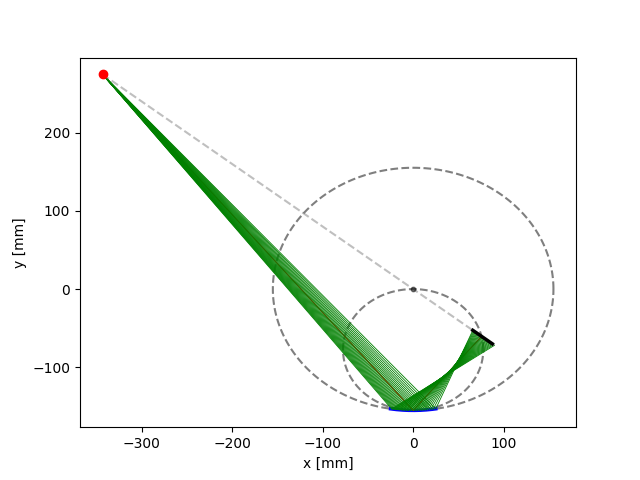
\includegraphics[width=0.9\textwidth]{Diagrams/FSSRsimpleRayTracing.png}
	\caption{Simple ray tracing of the FSSR-1D with 
	a mica 
	crystal with second order diffraction, where $R = 
	155$ 
	\unit{mm}, $E_0 = 1600$ \unit{eV} and $a_0 = 
	549.7$ 
	\unit{mm}. The detector 
	length in dispersive direction is 27.6 \unit{mm} and the 
	crystal length is 
	50 \unit{mm}. The red dot represents the source 
	and the red ray is the central ray. The remaining rays are 
	shown in green 
	The crystal is in blue and the detector in black. The dotted 
	circles depict 
	the crystal curvature and the RC respectively. Finally, the 
	black dot shows 
	the center of the crystal curvature circle.}
	\label{FSSRSimpleRayTracing}
\end{figure}

The code delivers the diagram seen in fig. 
\ref{FSSRSimpleRayTracing}, where 
the parameters of the final FSSR-1D are used. 
Notably, the 
detector line 
lies exactly on a symmetry axis of the circle drawn out from the 
crystal 
curvature, even though no explicit symmetry relations were used 
in the 
calculations. This supports the optimal orientation outlined in 
section \ref{section:dispersion calculation}. In 
addition, the angle of the central ray to the detector line is 
$90\degree$, as   
expected for the FSSR-1D geometry.

To note is that this geometry has many degrees of freedom when fine tuning the 
spectrometer. As such, it's simpler to set a parameter first, then adjust the 
others accordingly. In this work, I set the central ray to be incident on the 
center of the crystal, meaning the central energy $E_0$ corresponding to this 
ray doesn't lie in the center of the energy range due to the off-axis source 
location (relative to the spherical crystal optical axis). Therefore, the 
easiest way to fine tune the energy range, limited by detector position and 
size as well as crystal position and size, is to slightly shift the detector 
location along the symmetry axis mentioned above. In this case, I chose the top 
end of the detector (positive y direction) to correspond with the topmost ray 
(lowest energy ray) reflected from the crystal, as seen in fig. 
\ref{FSSRSimpleRayTracing}. This choice covered the largest 
possible energy range with this setup. With the offset and 
orientation set, the placement of the detector is determined. 

This code is applicable for all FSSR geometries and can be used 
to quickly 
determine the optimal detector placement for any FSSR. 

\section{Simulation of the Focusing Spectrograph with 
Spatial Resolution}
\label{section: FSSR simulation}
I simulated the FSSR-1D with the same parameters as in the final 
design (see table \ref{Table: Specs}) using 
mmpxrt. In this section I will discuss the quantities relevant 
to the 
validation of the final design. For more details about each 
graph and result of 
the simulation, refer to \citep{vsmid2021x}. 

\begin{figure}[H]
	\centering
	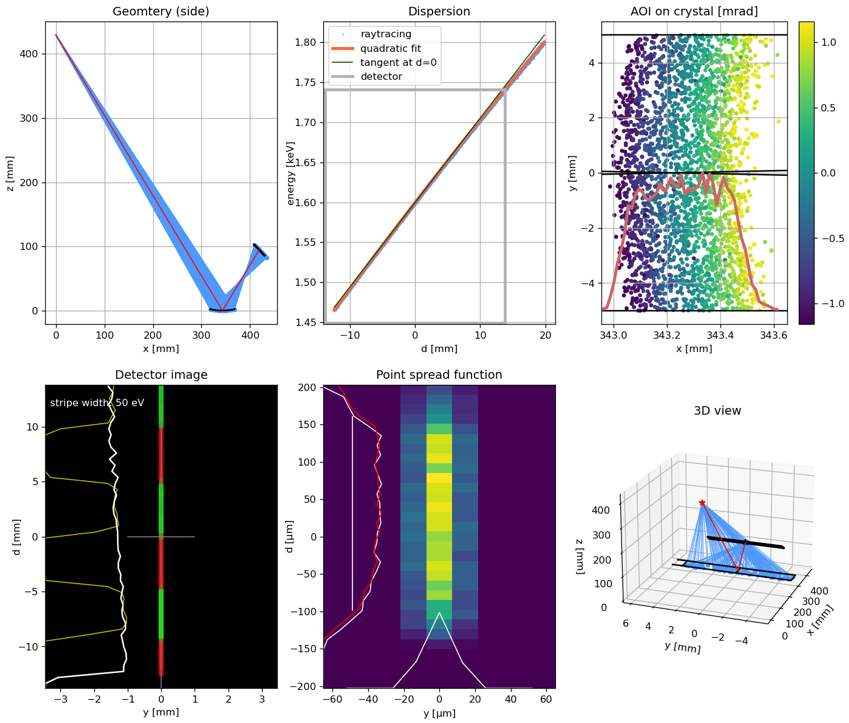
\includegraphics[width=\textwidth]{Diagrams/FSSRmmpxrtGraphs.PNG}
	\caption{Graphical results of mmpxrt simulation 
	of the FSSR-1D, wherein the point 
		spread function used to find the energy 
		resolution is in the bottom middle.}
	\label{mmpxrtFSSRGraphs}
\end{figure}

\begin{figure} [H]
	\begin{subfigure}[t]{0.37\textwidth}
	\centering
		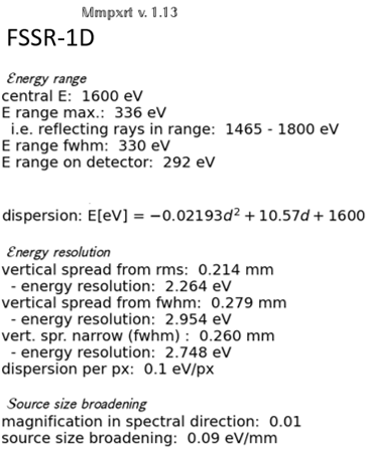
\includegraphics[width=\textwidth]{Diagrams/FSSRmmpxrtData.PNG}
		\caption{Numerical results of mmpxrt 
		simulation of FSSR-1D with some 
		quantities removed for clarity.}
		\label{mmpxrtFSSRData}
	\end{subfigure}%
	\hfill
	\begin{subfigure}[t]{0.68\textwidth}
	\centering
		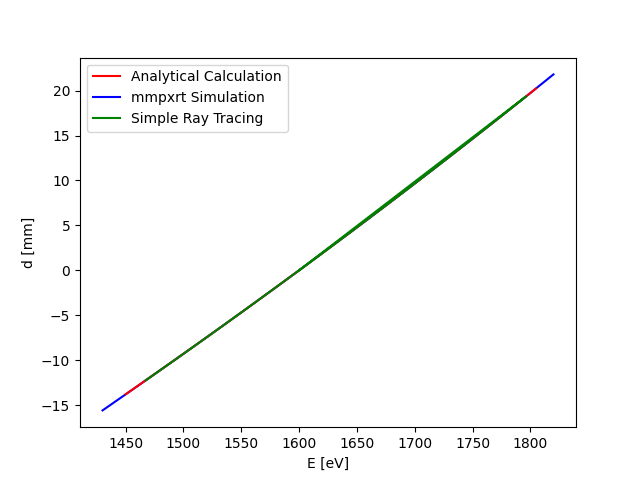
\includegraphics[width=\textwidth]{Diagrams/DispersionComparisonFSSR.png}
		\caption{Dispersion of the FSSR-1D calculated 
		with three 
		different methods.}
		\label{DispComparisonFSSR}
	\end{subfigure}%
	\caption{(a): Results of simulation of 
	the FSSR-1D with the parameters as in 
	fig. \ref{FSSRSimpleRayTracing}. Simulated using 
	mmpxrt \citep{vsmid2021x}. (b): Comparison of 
	dispersion. Energy range was extended for the 
	simple ray tracing and analytical results to 
	render them visible on the graph. }
	\label{mmpxrtFSSR}
\end{figure}

To run the ray tracing simulation, a number of parameters needed 
to be input. 
These include the geometry dependent parameters like radius of 
crystal 
curvature and source-crystal distance, among others, along with 
settings 
pertaining to the simulation and source/crystal 
properties. I set the simulation settings according 
to limitations 
of the computer 
and code, where the most important is the parameter 
p['simulation']['numerical\_intersect\_halving']=1, which 
increases the runtime 
but is necessary for simulating curved crystals. As for the 
source and crystal 
properties, I set the source to be a cube with length of 0.1 
\unit{mm} and the 
crystal as a monocrystal with a rocking curve width of 
\SI{2322}{\micro\radian}
and an integrated reflectivity of 
\SI{28.9}{\micro\radian}, as typical values for mica
\citep{holzer1998flat}.



To assess the accuracy of the simulation, I will first 
look at the dispersion. I determined the dispersion using three 
different 
techniques and graphed them together in fig. 
\ref{DispComparisonFSSR}. The 
simple ray tracing calculation was done by finding $d$ through 
the absolute 
distance between the imaging points of a given ray and the 
central ray. This is 
an excellent approximation, as the detector line 
follows the line of 
imaging points 
almost exactly, with negligibly small deviations on 
the order of 
$10^{-13}$\,\si{\milli\meter}. 
For the analytical calculation I used the relation in eq. 
\ref{DispersionCalcFSSR}. The simulation dispersion is found in 
fig. 
\ref{mmpxrtFSSRData}, where one need only take the 
inverse. It's 
immediately clear 
that the results show extremely good agreement. In fact, the 
lines overlap 
almost perfectly. This speaks for the validity of all three 
methods. 
Furthermore, the dispersion is, as desired, approximately 
linear over the energy range covered by the detector, 
as apparent 
in the fit of the analytical formula 
\begin{equation}
d(E) = 1.932\cdot 
10^{-5}\,\si{\milli\meter\per\electronvolt\squared} \cdot E^2 
+ 0.03292\,\si{\milli\meter\per\electronvolt} \cdot E - 102.1 
\,\si{\milli\meter} + \mathcal{O}(E^3).
\end{equation}

The simulation recovers an energy range of 1465 - 
1757\,\si{\electronvolt}, 
which is comparable to the range expected from the FSSR-1D 
design of 
approximately 1465 - 1755\,\si{\electronvolt}. Additionally, the 
dispersion per pixel, using a pixel size of 
\SI{13.5}{\micro\meter}, is 
reasonable when 
compared to the estimated value of \SI{0.14}{\electronvolt\per 
pixel} from the 
analytical 
formula. The magnification in dispersive direction 
and source size broadening 
are also as 
expected, taking negligibly small values, with the 
source broadening resulting in $\Delta E = 
$\SI{0.014}{\electronvolt}, assuming a source size of 
\SI{150}{\micro\meter}.

Before discussing the energy resolution, an 
explanation of each type of resolution given in the 
mmpxrt results is useful (see fig. 
\ref{mmpxrtFSSRData}). Each of the three resolutions 
given is derived from the point spread function (PSF) 
seen in fig. \ref{mmpxrtFSSRGraphs} using different 
methods. The first value from "vertical spread from 
rms" is calculated by taking the root-mean-square of 
the spread of points in the d direction, then 
multiplying a factor onto it to approximate a 
gaussian profile. Consequently, this value is not of 
much immediate use in this work, as it assumes a 
distribution. The second value from "vertical spread 
from fwhm" corresponds to the FWHM of the plot of the 
profile in dispersive (d) direction, integrating over 
the y direction. As such, this resolution takes into 
account the full y range shown in the PSF graph. The 
third value from "vert. spr. narrow (fwhm) uses the 
same process as the second value, with the exception 
of using only the y range shown by two red lines in 
the PSF graph. In summary, the first value will not 
be used in this work, while the choice between the 
second and third value depends on the y range on the 
detector one wishes to cover. It is important to 
mention that this energy resolution result takes only 
the crystal quality into account.

In the case of the FSSR-1D, the most instructive 
energy resolution is the second one, as the detector 
is large enough in the vertical direction 
(\SI{6.9}{\milli\meter}) to capture all the rays in 
the PSF graph. The result $\Delta E = 
2.954$\,\si{\electronvolt} is comparable to an 
estimated value of $\Delta E_{est} = 
2.960$\,\si{\electronvolt}, calculated from the 
rocking curve width $\Delta\theta =$ 
\SI{2322}{\micro\radian} with the formula
\begin{equation}
	\Delta E_{est} = E(\theta_0) - E(\theta_0 + 
	\Delta\theta),
	\label{eq: energy resolution estimate}
\end{equation}
where $E(\theta)$ is determined using Bragg's law 
(see eq. \ref{Bragg}). The agreement between the 
estimated and simulated value speaks for the 
trustworthiness of the result. To note is that this 
energy resolution depends directly on the crystal 
quality, and 
as such can be noticeably different in the experiment.

\section{Simulation of the Dual Unbent Crystal 
Spectrometer}
\label{section: DUCC Simulation}
As with the FSSR-1D, I simulated the DUCC using the 
parameters as 
in the design (see section \ref{section:DUCC 
design}), where only one 
channel was 
considered, as the geometry is analogous along both channels. 

The source and simulation parameters in mmpxrt were set just as 
in section \ref{section: FSSR simulation}, 
with the exception of leaving out the 
"numerical\_intersect\_halving" parameter, 
since the crystal is flat. The geometry parameters were chosen 
as in the actual 
design (see table \ref{Table: Specs}). The crystal 
properties were chosen to 
correspond to a 
monocrystal with an integrated 
reflectivity 
of \SI{2.32}{\micro\radian}, taken from 
\citep{ferrari2019characterization}, and 
rocking curve width of \SI{800}{\micro\radian}, which 
was artificially increased from the literature value 
of 
\SI{165}{\micro\radian} \citep{rajesh2015growth}, since the 
simulation did not 
function for too small a $\Delta \theta$, most likely owing to 
too few 
reflected rays.


\begin{figure}[H]
	\centering
	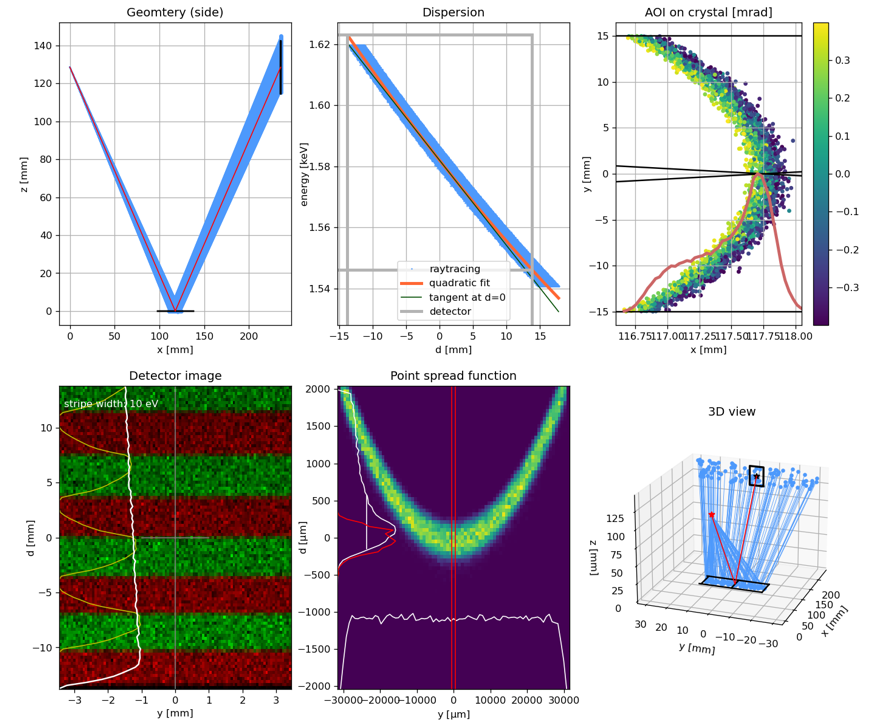
\includegraphics[width=\textwidth]{Diagrams/DUCCmmpxrtGraphs.PNG}
	\caption{Graphical results of mmpxrt simulation 
	of the DUCC, wherein the point 
		spread function used to find the energy 
		resolution is in the bottom middle.}
	\label{mmpxrtDUCCGraphs}
\end{figure}

\begin{figure} [H]
	\begin{subfigure}[t]{0.37\textwidth}
	\centering
		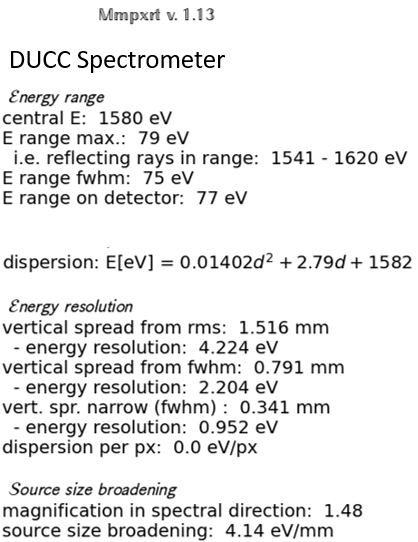
\includegraphics[width=\textwidth]{Diagrams/DUCCmmpxrtData.PNG}
		\caption{Numerical results of mmpxrt 
		simulation of DUCC with some 
		quantities removed for clarity.}
		\label{mmpxrtDUCCData}
	\end{subfigure}%
	\hfill
	\begin{subfigure}[t]{0.68\textwidth}
	\centering
		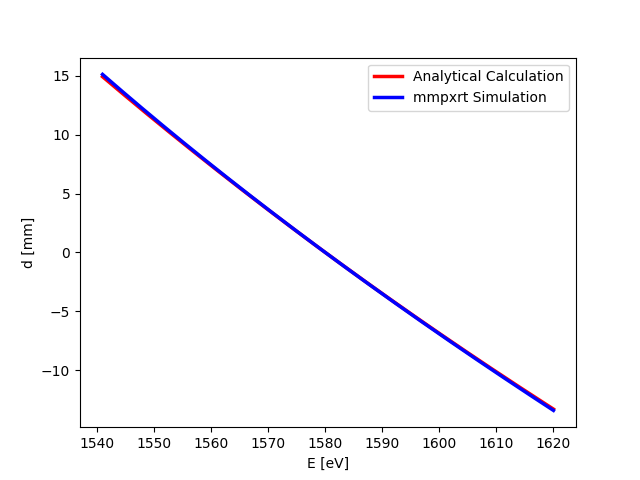
\includegraphics[width=\textwidth]{Diagrams/DispersionComparisonDUCK.png}
		\caption{Dispersion of the DUCC calculated 
		with two different methods.}
		\label{DispComparisonDUCK}
	\end{subfigure}%
	\caption{(a): Results of simulation of 
	the DUCC with the parameters as in 
	table \ref{Table: Specs}. Simulated using 
	mmpxrt \citep{vsmid2021x}. (b): Comparison of 
	dispersion calculated analytically and 
	through the mmpxrt simulation.}
	\label{mmpxrtDUCC}
\end{figure}

As before, the dispersion $d(E)$ is determined using different 
methods, namely 
by the simulation and analytically using eq. 
\ref{DispersionCalcDUCK}. The 
results are pictured in fig. \ref{DispComparisonDUCK}, where 
again a very good 
agreement is apparent. In this case the dispersion is also 
approximately 
linear, albeit less than for the FSSR-1D, with a fit 
of the 
analytical 
equation resulting in 
\begin{equation}
d(E) = 6.306\cdot 
10^{-4}\,\si{\milli\meter\per\electronvolt\squared} \cdot E^2 
-2.35\,\si{\milli\meter\per\electronvolt} \cdot E - 2139 
\,\si{\milli\meter} + \mathcal{O}(E^3).
\end{equation}

The energy range as well shows good agreement, with ranges of 
1541 - 
1618\,\si{\electronvolt} for the simulation and approximately 
1541 - 
1620\,\si{\electronvolt} for the design. The dispersion per 
pixel is also as 
expected, with 0.037\,\si{\electronvolt\per pixel} for the 
analytical 
dispersion taking into account the pixel size of 
\SI{13.5}{\micro\meter}, which 
is low 
enough to display as 0.0\,\si{\electronvolt\per pixel} in the 
simulation.

In the case of the source broadening, the 
simulation results slightly deviate from the 
analytically 
estimated value. This estimate assumes a 
source size in 
the dispersive plane of \SI{150}{\micro\meter} and 
uses 1-to-1 imaging of a 2D source onto the detector, 
which follows from the 
geometry and the fact that source extension in the 
vertical direction should not affect spectral 
resolution. Together with the dispersion, this 
delivers a broadening of \SI{0.592}{eV}, while the 
simulation gives a value of 
$\SI{4.14}{\electronvolt\per\milli\meter}\cdot 
\SI{0.15}{\milli\meter} = \SI{0.621}{\electronvolt}$. 
The deviation can be possibly traced back to 
the way that mmpxrt handles the source broadening 
calculation, which is done using a monochromatic ray 
tracing, where an offset of the source is 
introduced for some rays \citep{vsmid2021x}. 
Accordingly, the source broadening becomes dependent 
on the crystal quality. The artificially increased 
rocking curve width therefore leads to higher values 
of the source broadening in the code. Despite this, 
the simulation value will be carried over, as the 
estimate is fairly coarse.

For the energy resolution, as opposed to the FSSR-1D, 
the third value in fig. \ref{mmpxrtDUCCData} is used, 
as the detector only covers a fraction of the y range 
in the PSF graph, so that $\Delta E = 
$\SI{0.952}{\electronvolt}, while the formula to 
estimate the spectral resolution from the rocking 
curve width (see eq. \ref{eq: energy resolution 
estimate}) yields $\Delta E_{est} = 
$\SI{0.238}{\electronvolt}. Due to the artificial 
increase of $\Delta\theta$ in the simulation, $\Delta 
E_{est}$ will be used instead of $\Delta E$ in this 
work.


\section{Summary of Simulation Results}
\label{section: simulation results}
For both the DUCC and FSSR-1D spectrometers, the mmpxrt 
simulations yielded 
results consistent with the analytical calculations, 
showing very good 
agreement for the 
dispersion, dispersion per pixel and energy range, 
and good agreement for source broadening. The 
energy resolution agreed well for the FSSR-1D, while 
the $\Delta E_{crystal}$ from the DUCC simulation is 
not 
meaningful due to the artificially increased 
$\Delta\theta$.

Since one of the main goals of the simulations was assessing the 
spectral 
resolution of each spectrometer, I have gathered and presented 
the 
contributions to the resolutions in table 
\ref{TableResolutions}, along with the total spectral 
resolution $\Delta E_{tot}$ calculated by summing all 
the results. 

It is immediately clear that the crystal properties 
are the main limiting factor on the resolution for 
the FSSR-1D, while the DUCC resolution is mostly 
limited 
by the source broadening, with a significant, though 
smaller, contribution from the rocking curve width. 
Here we see the advantage offered by the ADP crystal 
in comparison to the mica, in that it delivers better 
spectral resolution, albeit at the cost of lower 
integrated reflectivity and worse bendability. These 
results also indicate that the detector 
resolution does not limit the overall spectral 
resolution for either spectrometer. In general, both 
spectrometers have sufficient 
spectral resolutions to perform their roles outlined 
in section \ref{section: spectrometer geometries}.

\begin{table}[H]
\centering
\caption{Resolution contributions for the DUCC and FSSR-1D 
spectrometers. 
 In both cases, the source broadening is taken from 
 mmpxrt and assumes a source size of 
 \SI{150}{\micro\meter}, and the detector resolution 
 is calculated from the mmpxrt dispersion and uses a 
 pixel size of \SI{13.5}{\micro\meter}. The 
 contribution due to the crystal properties for the 
 DUCC is estimated as described in section 
 \ref{section: DUCC Simulation}, while for the 
 FSSR-1D it is taken from mmpxrt's second $\Delta E$ 
 value. The total spectral resolution is calculated by using error propagation 
 on the source broadening and crystal properties' resolution, then linearly 
 adding on the detector resolution.}
\vspace{0.05cm}
\renewcommand{\arraystretch}{1.5}
\centering
\begin{tabular}{|c|c|c|} 
\hline
$\Delta E$ Contributions & DUCC 
& FSSR-1D \\ [0.5ex]
\hline\hline
Source Broadening & \eV{0.621} & \eV{0.014} \\ 
[0.5ex]
\hline
Detector & \eV{0.038} & \eV{0.143} \\ [0.5ex]
\hline
Crystal Properties & \eV{0.238} & \eV{2.954} \\ 
[0.5ex]
\hlineB{7}
Total & \eV{0.703} & \eV{3.097} \\ [0.5ex]
\hline
\end{tabular}
\label{TableResolutions appendix}
\end{table}

\chapter{Alignment Procedure for FSSR-1D}
\label{section: FSSR-1D alignment}

The alignment process can be broken down into 5 steps. To note is that parts of 
the alignment are built into the mechanical design itself, such that manual 
adjustments are not required. I will touch on these aspects after explaining 
the procedure. 

Essential to the alignment are the four optical stages labeled in fig. 
\ref{InvFSSRAlignment}. The rotation stage is a PR01/M, the large 
linear stage a LX10/M, and the tip-tilt stage a KM100B/M from 
\textit{Thorlabs}. The fine linear stage, a TSDS-1 from 
\textit{SigmaKoki}, serves to adjust the crystal-pin distance and the 
tip-tilt stage allows for pointing in step 2. 

The first three steps are conducted outside the target chamber on an optical 
table equipped with an expanded collimated laser beam, in our case a 
HeNe laser, while the last two steps are carried out in 
the chamber.

\begin{enumerate}
	\item First, the FSSR-1D without the crystal apparatus is brought into 
	alignment with the HeNe beam for the next steps, simultaneously ensuring 
	that the spectrometer 
	base plate lies parallel to the floor. The HeNe beam is directed onto the 
	opening of the front plate, onto which a pin is affixed, as seen in 
	fig \ref{InvFSSRAlignment11}. The shadow cast by the pin is then 
	aligned with the center of 
	the cross on a plate attached to the back of the base of the 
	FSSR-1D (see fig. \ref{InvFSSRAlignment12}). In this way the beam 
	is parallel to the base plate of the FSSR-1D and to the line drawn 
	out from the pin to the rotation axis of the rotation stage.
	\item Now the crystal apparatus, consisting of the rotation stage, 
	fine linear stage, tip-tilt stage and the crystal holder, is put 
	in, as seen in fig. \ref{InvFSSRAlignment21}. Using the fine linear 
	stage and tip-tilt stage, the beam is 
	focused with the crystal onto the 
	surface of the pin (see fig. \ref{InvFSSRAlignment22}), whose 
	distance to the crystal is exactly the 
	focal length of the crystal. This 
	serves to set the location of the Rowland circle 
	and ensure that the crystal center intersects the rotation axis of 
	the rotation stage. It also corrects for any unintended tilts or 
	shifts of the crystal w.r.t the rest of the spectrometer. 
	\item Next, the central Bragg angle is set by rotating the crystal 
	with the rotation stage. This step leaves the crystal in its final 
	position (see fig. \ref{InvFSSR}). In preparation for the next 
	step, the pin is removed 
	and the pointer holder shown in fig. \ref{InvFSSRAlignment3} is 
	attached to the front of the front plate. Analogously to the DUCC, 
	an optical post is set to the required distance and screwed onto 
	the pointer holder.
	\item The pointer is then used to orientate the FSSR-1D in the 
	chamber. This is equivalent to fixing the $a_0$ 
	distance as defined in section \ref{SectionTheoryFSSR}.
	\item Finally, a laser is shone onto the tip of a needle placed at 
	the TCC. This 
	allows for taking images of the source with photons in the optical 
	range being reflected on the crystal and detected by the CCD camera 
	of the FSSR-1D. By adjusting the distance from chip to 
	crystal using the large linear stage under the camera pictured in 
	fig. \ref{InvFSSRAlignment12}, the position of best focus is found, 
	resulting in the thinnest possible horizontal line on the camera. 
	This is paramount to setting the 
	$b_0$ distance for the FSSR-1D geometry.
\end{enumerate}

With this the alignment is complete and the FSSR-1D geometry is realized. The 
most important mechanical details that assist in the alignment are as follows:
\begin{itemize}
	\item The rotation stage, front plate, cross plate (used in the first step) 
	and camera linear stage all lie in grooves in the base plate, which fixes 
	their locations and angles w.r.t one another. 
	\item Through additional positioning grooves for the pin and pointer 
	holder, the relative distances between every part is further preserved by 
	mechanical precision. In this way the distance from pin to rotation axis of 
	the rotation stage is set to the focal length of the spherical crystal, 
	allowing the second alignment step to line up the crystal center with the 
	rotation axis. 
	\item Finally, the crystal holder and corresponding connections to the 
	stages ensure that the crystal lies at the correct height and parallel to 
	the base plate, carrying over the alignment achieved in the first step. 
\end{itemize}

With this setup the error of the alignment is mostly limited to mechanical 
precision, excepting the fourth step, which relies on bare-eye precision. 
Despite this the overall precision remains excellent, as this uncertainty 
occurs relatively far from the spectrometer itself, reducing its 
impact.  

\begin{figure}[H]
	\centering
	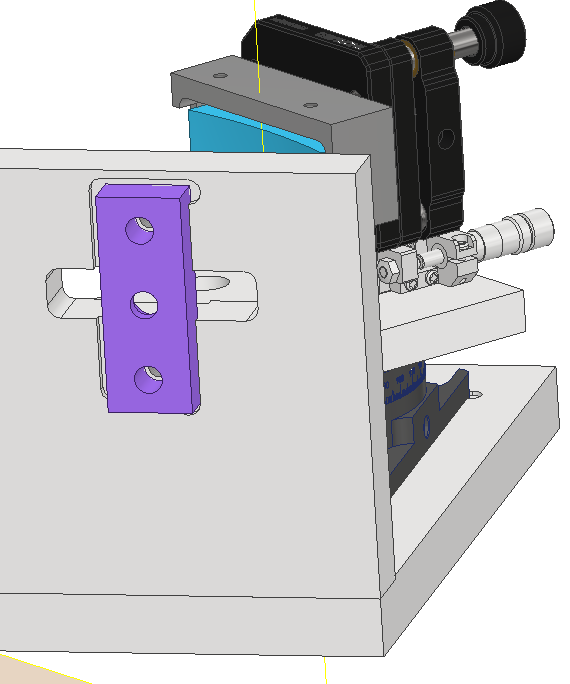
\includegraphics[width=0.4\textwidth]{InventorPics/Alignment3.PNG}
	\caption{Front view of step 3 depicting the pointer 
		holder set in 
		its groove in purple.}
	\label{InvFSSRAlignment3}
\end{figure}

\begin{figure} [H]
	\centering
	\begin{subfigure}[t]{0.42\textwidth}
		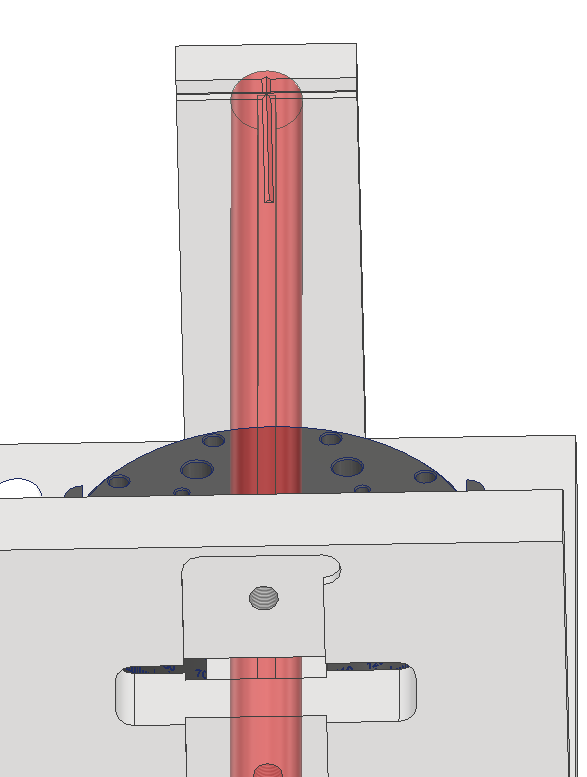
\includegraphics[width=\textwidth]{InventorPics/Alignment1.1.PNG}
		\caption{Top view of step 1. The HeNe beam is directed through 
		the front plate opening onto the cross plate.}
		\label{InvFSSRAlignment11}
	\end{subfigure}%
	\hfill
	\begin{subfigure}[t]{0.56\textwidth}
	\centering
		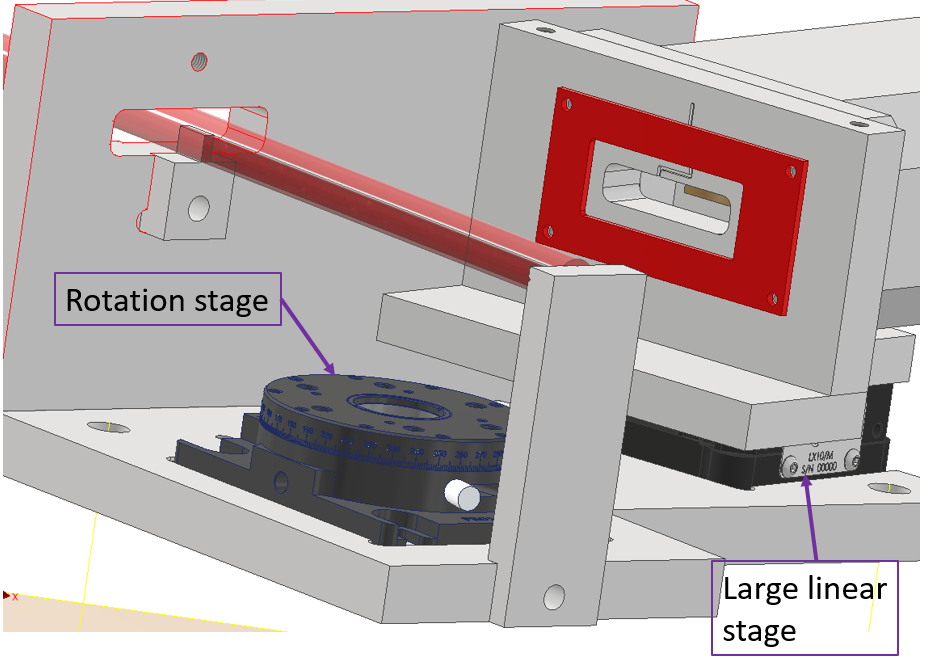
\includegraphics[width=\textwidth]{InventorPics/Alignment1.2.PNG}
		\caption{Back view of step 1, where the shadow of the pin is 
		visible in the HeNe beam. The rotation stage and large linear 
		stage are labeled.}
		\label{InvFSSRAlignment12}
	\end{subfigure}\\[1ex]
	\centering
	\begin{subfigure}[t]{0.48\textwidth}
	\centering
		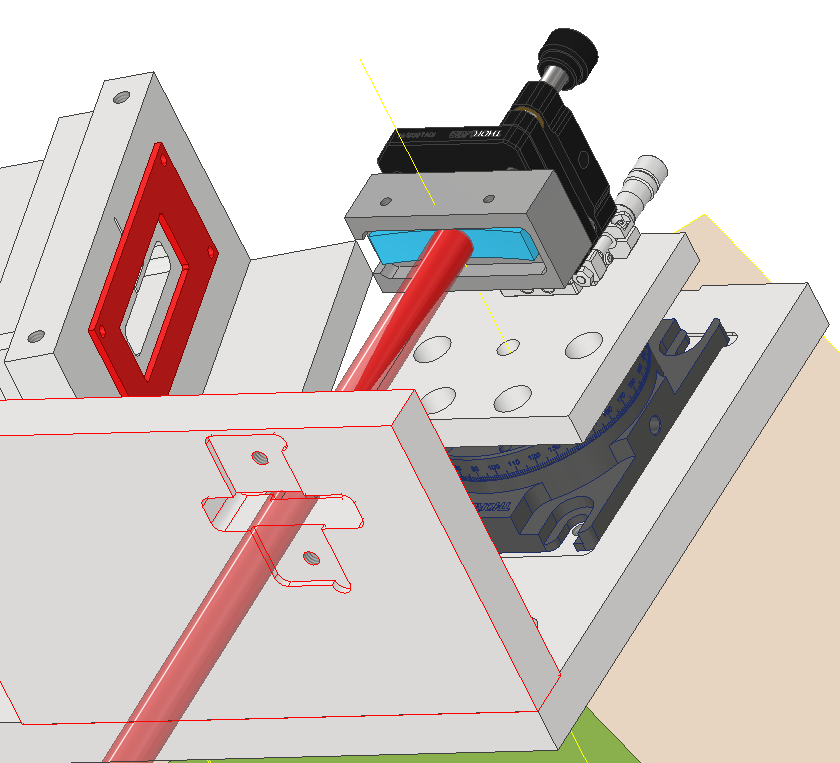
\includegraphics[width=\textwidth]{InventorPics/Alignment2.1.PNG}
		\caption{Front view of focusing in step 2. The focused HeNe 
		beam is depicted within the main beam in a darker red. The 
		rotation axis of the rotation stage is also shown.}
		\label{InvFSSRAlignment21}
	\end{subfigure}% 
	\hfill
	\begin{subfigure}[t]{0.48\textwidth}
	\centering
		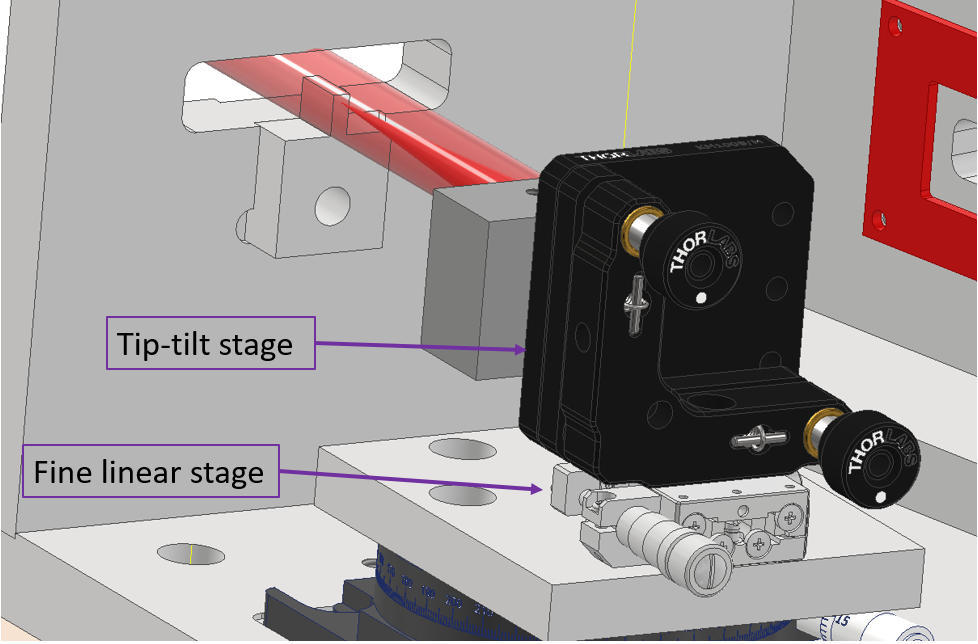
\includegraphics[width=\textwidth]{InventorPics/Alignment2.2.PNG}
		\caption{Back view of focusing in step 2. The tip-tilt and fine 
		linear stage are labeled.}
		\label{InvFSSRAlignment22}
	\end{subfigure}
	\caption{Model depicting the alignment process for the FSSR-1D 
	using a collimated HeNe laser, which is shown in red. The various 
	optical stages are labeled.}
	\label{InvFSSRAlignment}
\end{figure}

\chapter{Supplementary Results}
\label{appendix: supplementary results}


\section{Spectral Resolution}
\label{appendix: spectral resolution}

\begin{figure} [H]
	\centering
	\begin{subfigure}[t]{0.49\textwidth}
		\centering
		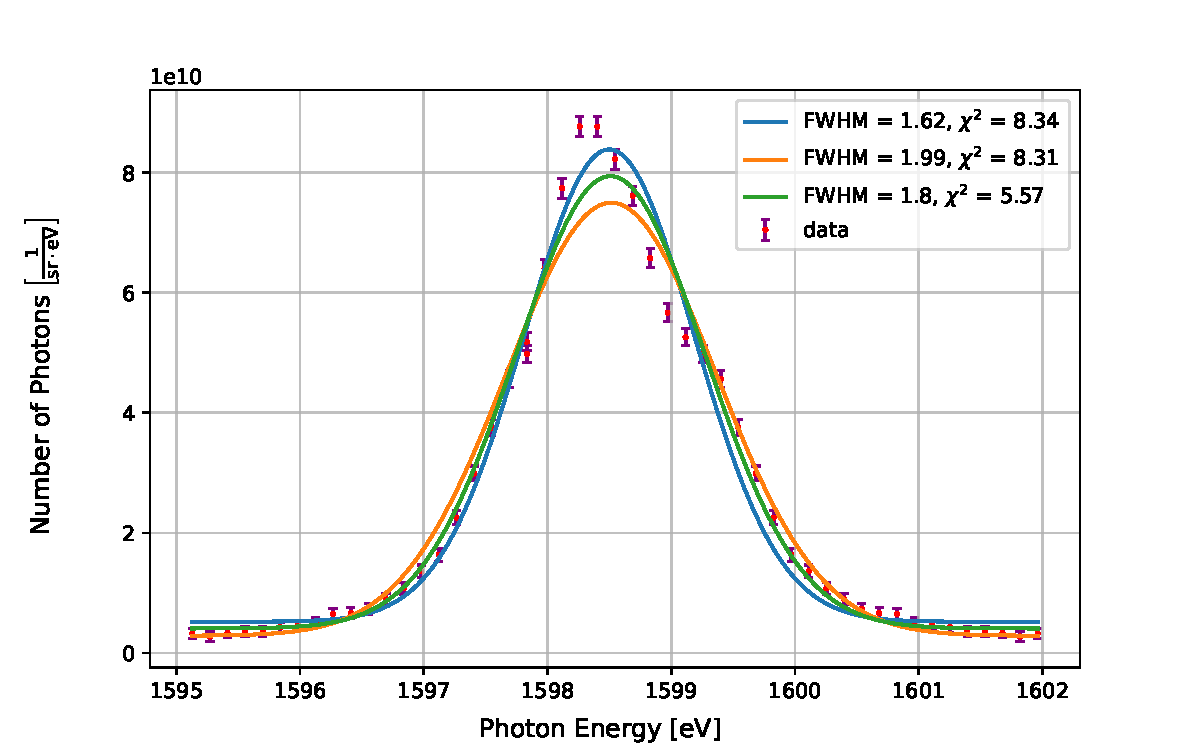
\includegraphics[width=\textwidth]{Data_Analysis/resolution/peak_of_Al_event_2_on_FSSR.pdf}
		\caption{FSSR: Gaussian fit of the He-$\upalpha$ line for a \SI{1.7}{\joule} shot on aluminum (event 2).}
		\label{}
	\end{subfigure}%
	\hfill
	\begin{subfigure}[t]{0.49\textwidth}
		\centering
		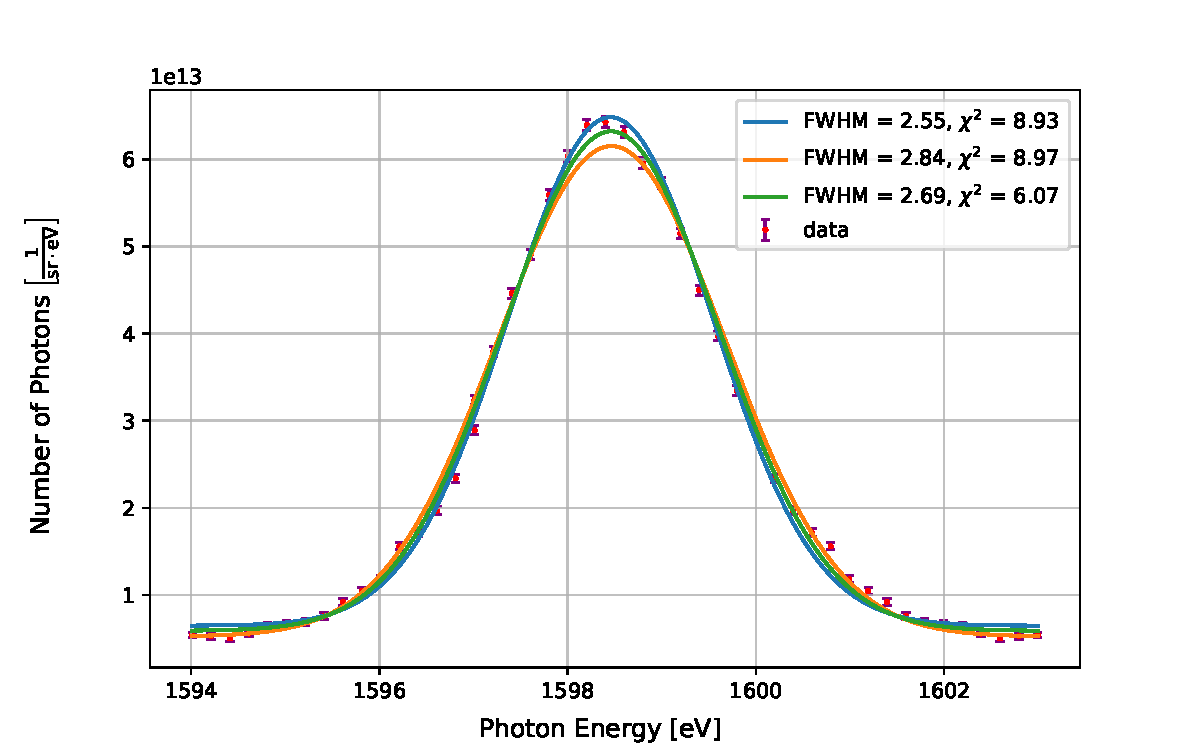
\includegraphics[width=\textwidth]{Data_Analysis/resolution/peak_of_Al_(thick)_event_16_on_SUCC.pdf}
		\caption{SUCC: Gaussian fit of the He-$\upalpha$ line for a \SI{24}{\joule} shot on aluminum (event 16).}
		\label{}
	\end{subfigure}
	\begin{subfigure}[t]{0.49\textwidth}
		\centering
		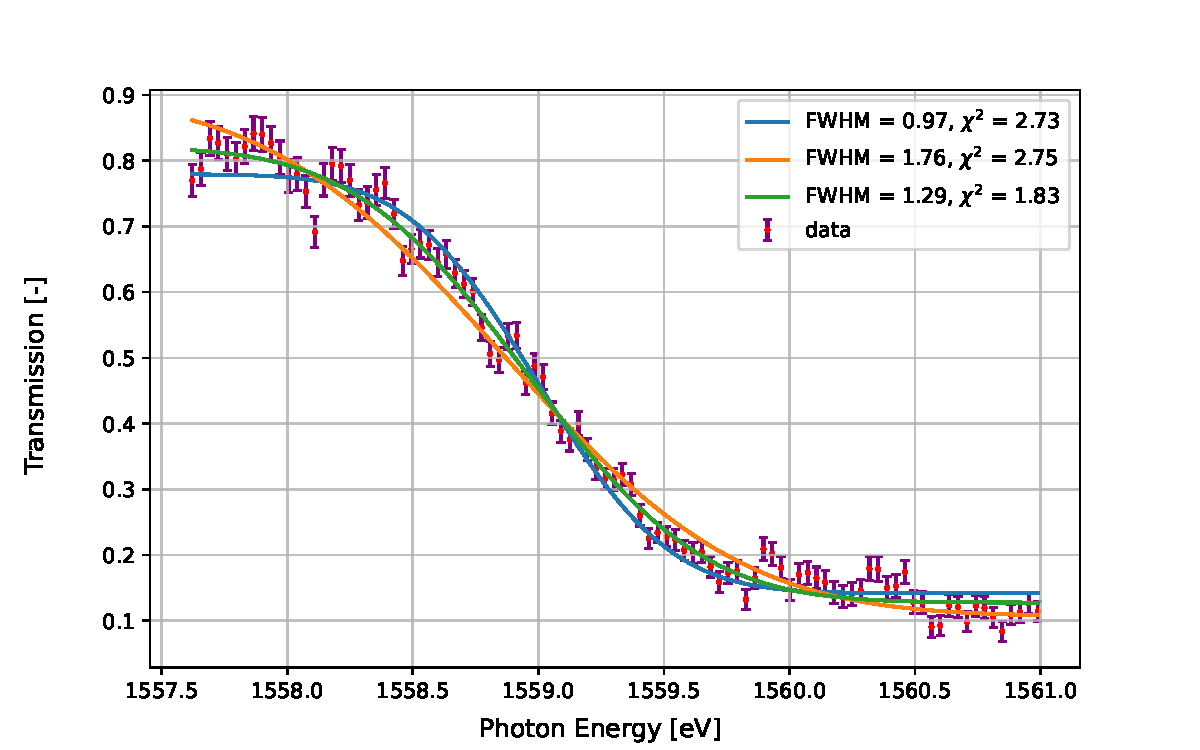
\includegraphics[width=\textwidth]{Data_Analysis/resolution/transmission_of_Sm_event_31_on_DUCC.pdf}
		\caption{DUCC: Error function fit of the transmission for a \SI{92.7}{\joule} shot on samarium (event 31).}
		\label{}
	\end{subfigure}%
	\hfill
	\begin{subfigure}[t]{0.49\textwidth}
		\centering
		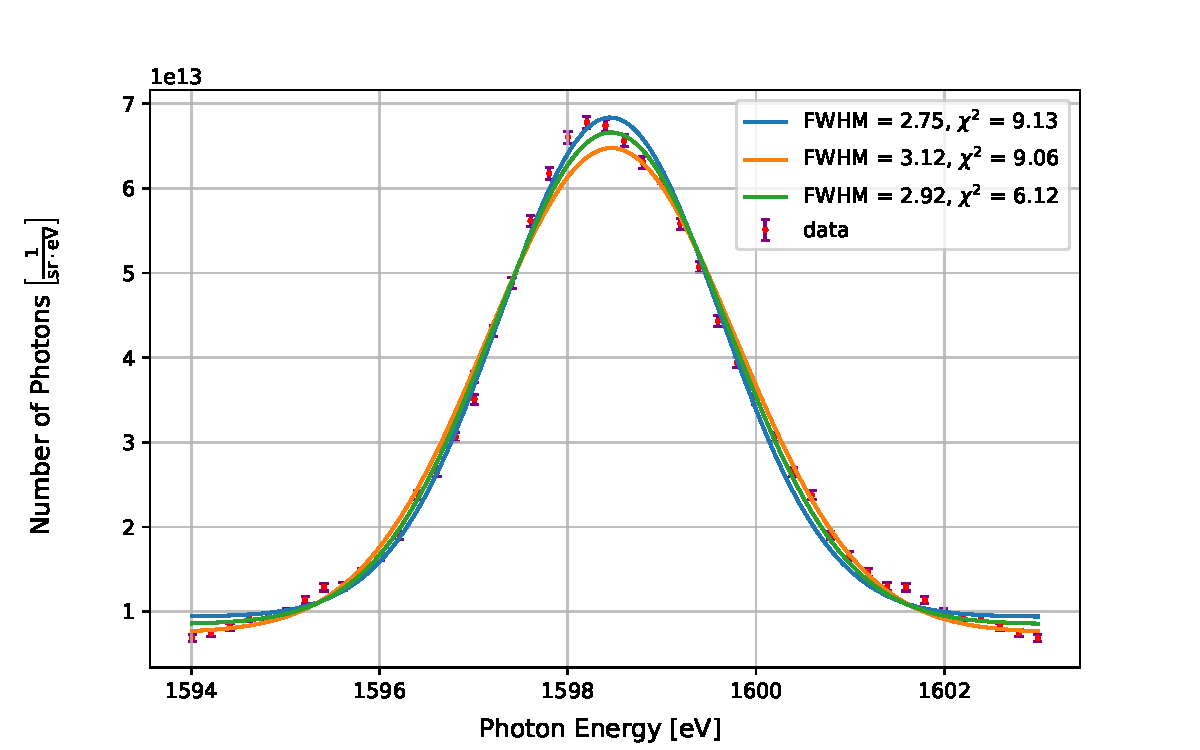
\includegraphics[width=\textwidth]{Data_Analysis/resolution/peak_of_Al_event_19_on_SUCC.pdf}
		\caption{SUCC: Gaussian fit of the He-$\upalpha$ line for a \SI{27}{\joule} shot on aluminum (event 19).}
		\label{}
	\end{subfigure}
	\caption{Fits used to determine the spectral resolution of various spectrometers. The best (green) and worst (blue and orange) fit models are depicted and labeled with their corresponding FWHM and $\chi^2$ values.}
	\label{}
\end{figure}

\section{Integrated Reflectivity Ratio}
\label{appendix: integrated reflectivity ratio}

\begin{figure}[H]
	\centering
	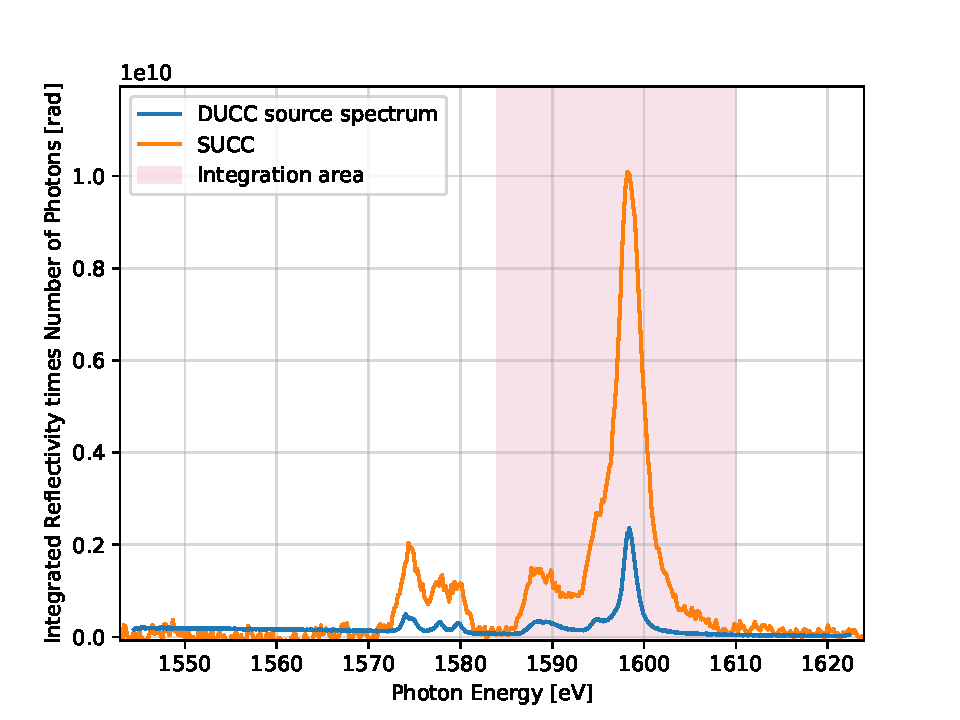
\includegraphics[width=0.6\textwidth]{Data_Analysis/R_int_ratio/spectra_of_Al_event_19_source.pdf}
	\caption{$R_{int}\cdot N_{total}$ for a \SI{27}{\joule} shot on aluminum (event 19). The spectra from the source channel of the DUCC and the SUCC are presented, as well as the integration area used to calculate the integrated reflectivity ratio.}
	\label{}
\end{figure}

\begin{figure}[H]
	\centering
	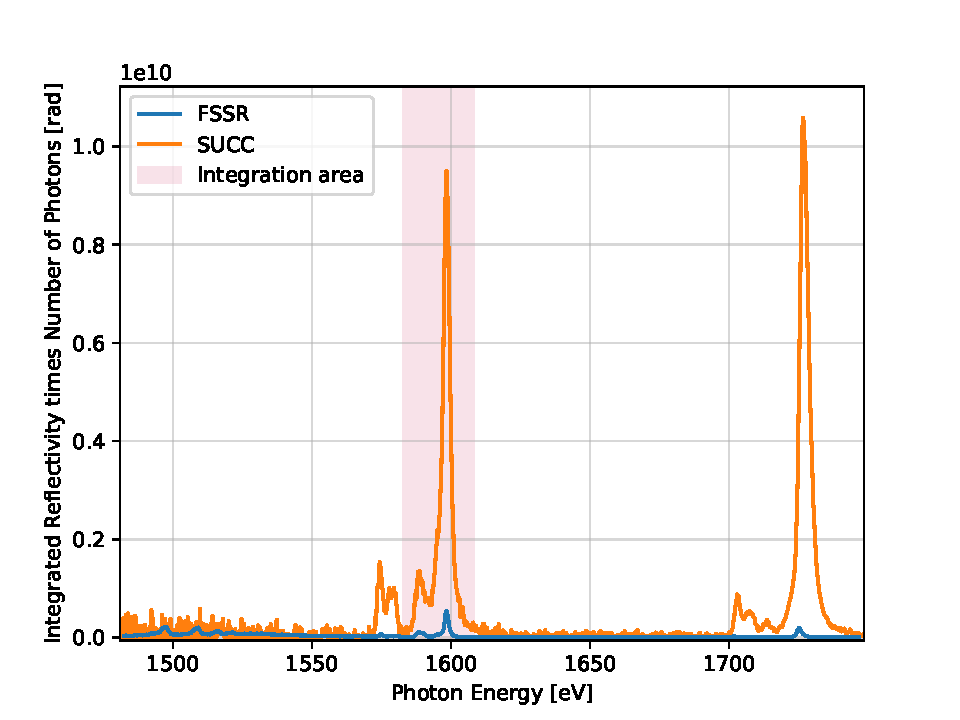
\includegraphics[width=0.6\textwidth]{Data_Analysis/R_int_ratio/spectra_of_Al_(thick)_event_16.pdf}
	\caption{$R_{int}\cdot N_{total}$ for a \SI{24}{\joule} shot on aluminum (event 16). The spectra from the FSSR and the SUCC are presented, as well as the integration area used to calculate the integrated reflectivity ratio.}
	\label{}
\end{figure}

\section{Conversion Efficiency into He-$\upalpha$ Emission Line of Aluminum}

\begin{figure} [H]
	\centering
	\begin{subfigure}[t]{0.49\textwidth}
		\centering
		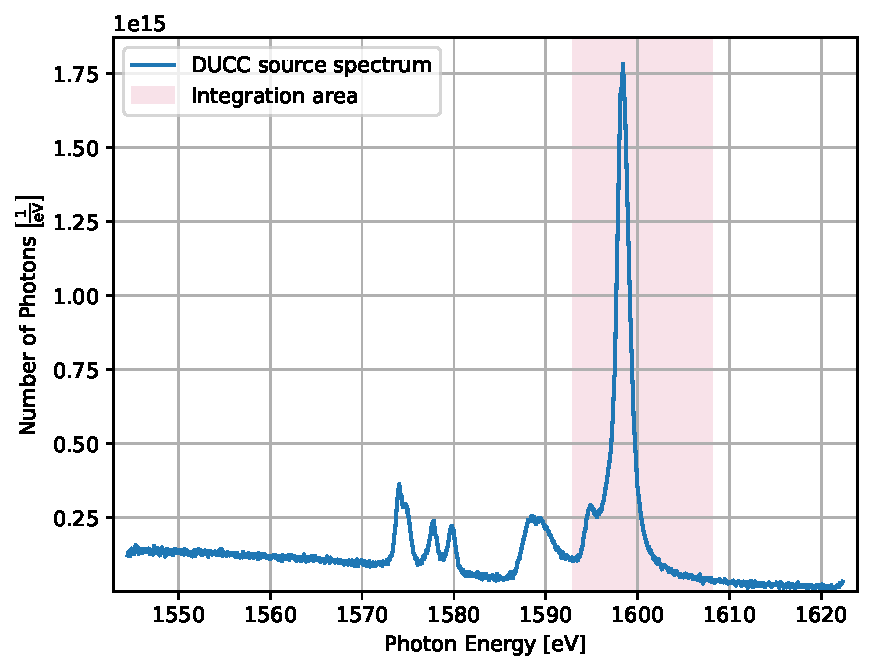
\includegraphics[width=\textwidth]{Data_Analysis/converison_efficiency/spectra_of_Al_event_19_on_DUCC_source_spectrum.pdf}
		\caption{DUCC source channel: Spectrum from a \SI{27}{\joule} shot on aluminum (event 19).}
		\label{}
	\end{subfigure}%
	\hfill
	\begin{subfigure}[t]{0.49\textwidth}
		\centering
		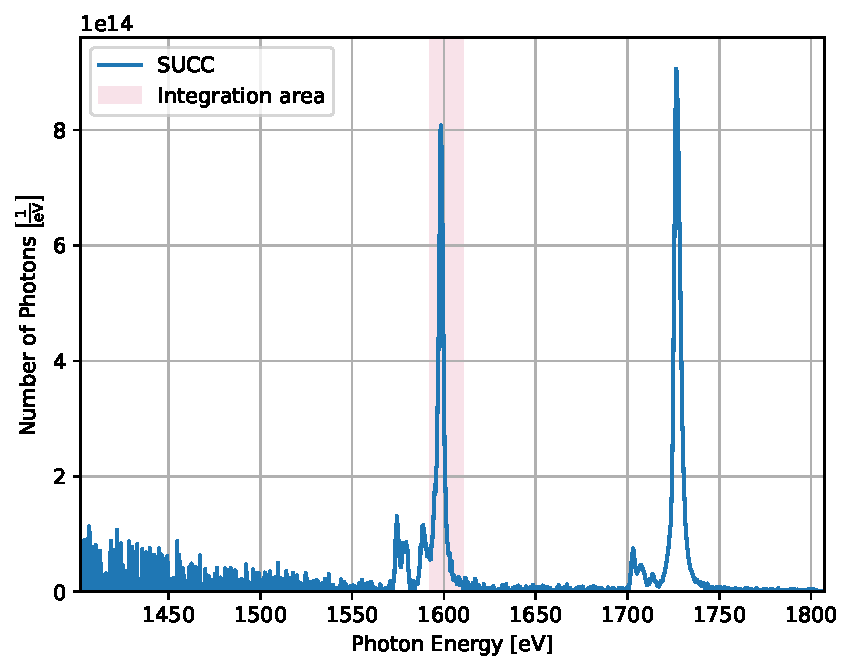
\includegraphics[width=\textwidth]{Data_Analysis/converison_efficiency/spectra_of_Al_(thick)_event_16_on_SUCC.pdf}
		\caption{SUCC: Spectrum from a \SI{24}{\joule} shot on aluminum (event 16).}
		\label{}
	\end{subfigure}
	\begin{subfigure}[t]{0.49\textwidth}
		\centering
		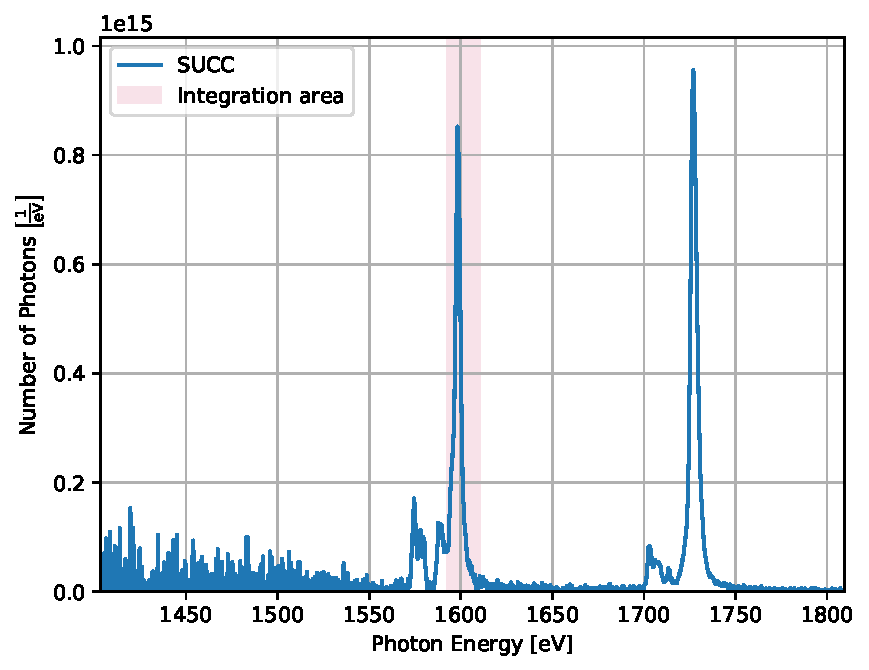
\includegraphics[width=\textwidth]{Data_Analysis/converison_efficiency/spectra_of_Al_event_19_on_SUCC.pdf}
		\caption{SUCC: Spectrum from a \SI{27}{\joule} shot on aluminum (event 19).}
		\label{}
	\end{subfigure}%
	\hfill
	\begin{subfigure}[t]{0.49\textwidth}
		\centering
		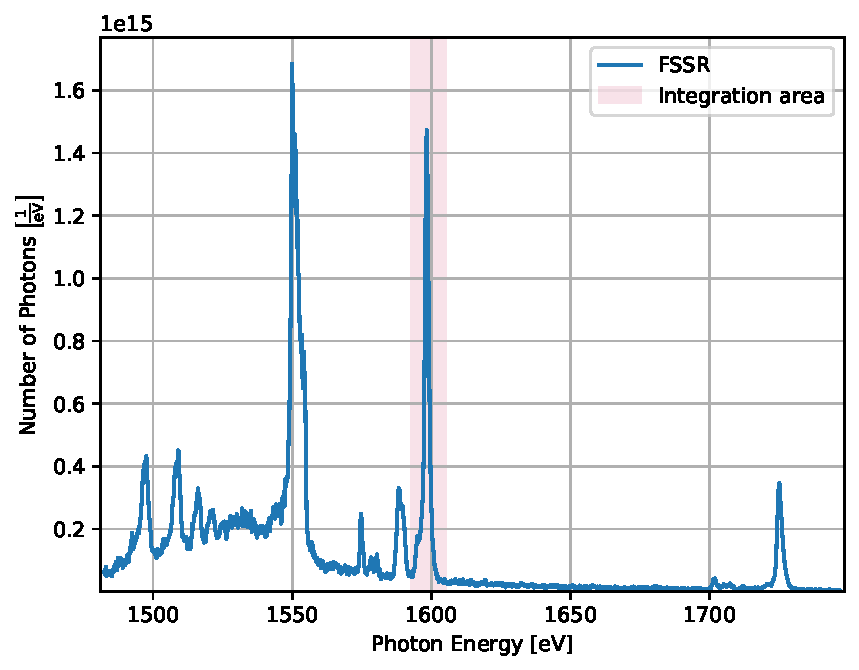
\includegraphics[width=\textwidth]{Data_Analysis/converison_efficiency/spectra_of_Al_(thick)_event_16_on_FSSR.pdf}
		\caption{FSSR: Spectrum from a \SI{24}{\joule} shot on aluminum (event 16).}
		\label{}
	\end{subfigure}%
	\caption{Spectra from various spectrometers utilized to determine the conversion efficiency. The area over which the signals belonging to the Al He-$\upalpha$ line are summed is depicted in pink.}
	\label{}
\end{figure}

\section{Additional Simulations}
\label{section: new simulations}

\begin{figure}[H]
	\centering
	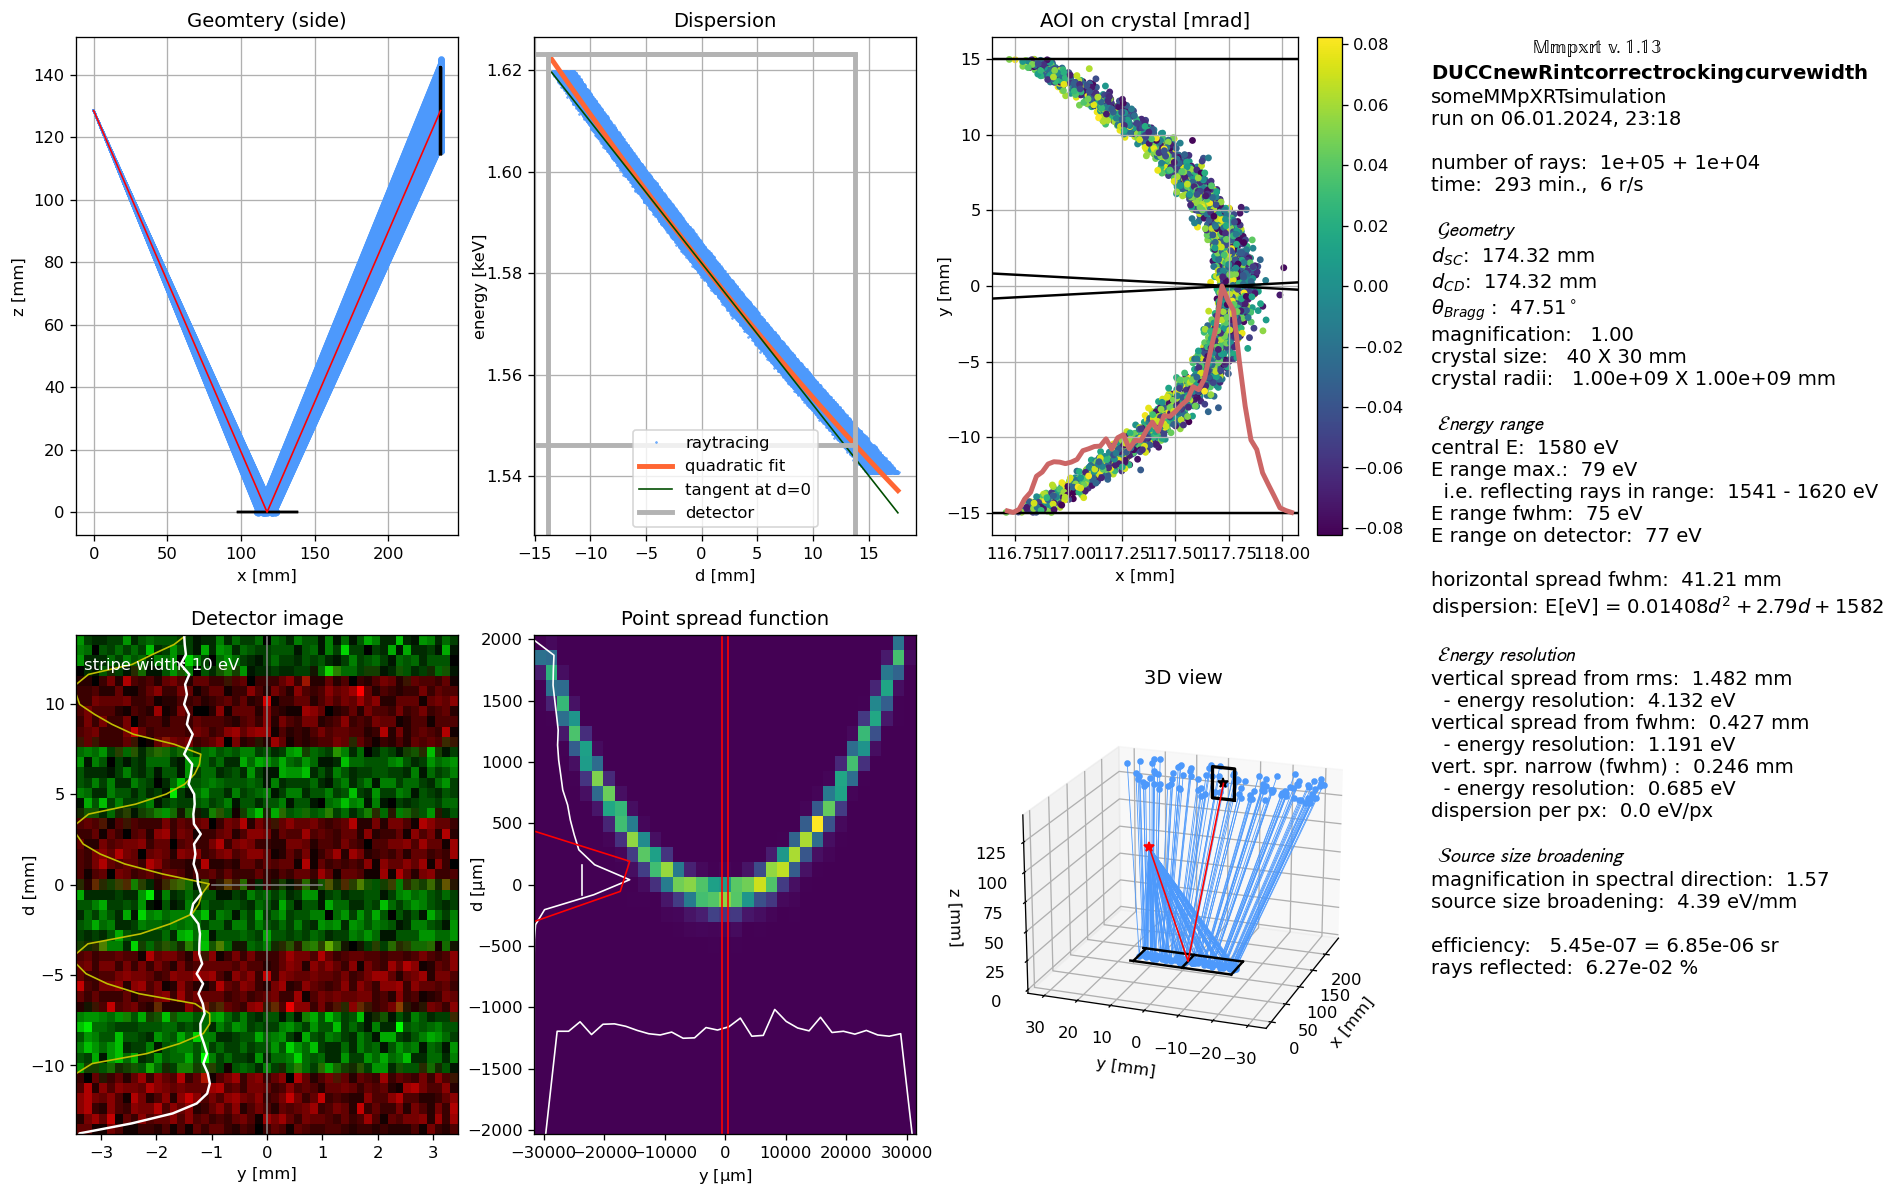
\includegraphics[width=1.12\textwidth, angle=90]{Data_Analysis/mmpxrt_DUCC_new_values.png}
	\caption{Results of \textit{mmpxrt} simulation of the DUCC with an integrated reflectivity of \SI{40}{\micro\radian} and a rocking curve width of \SI{165}{\micro\radian}}
	\label{fig: DUCC new mmpxrt}
\end{figure}

\begin{figure}[H]
	\centering
	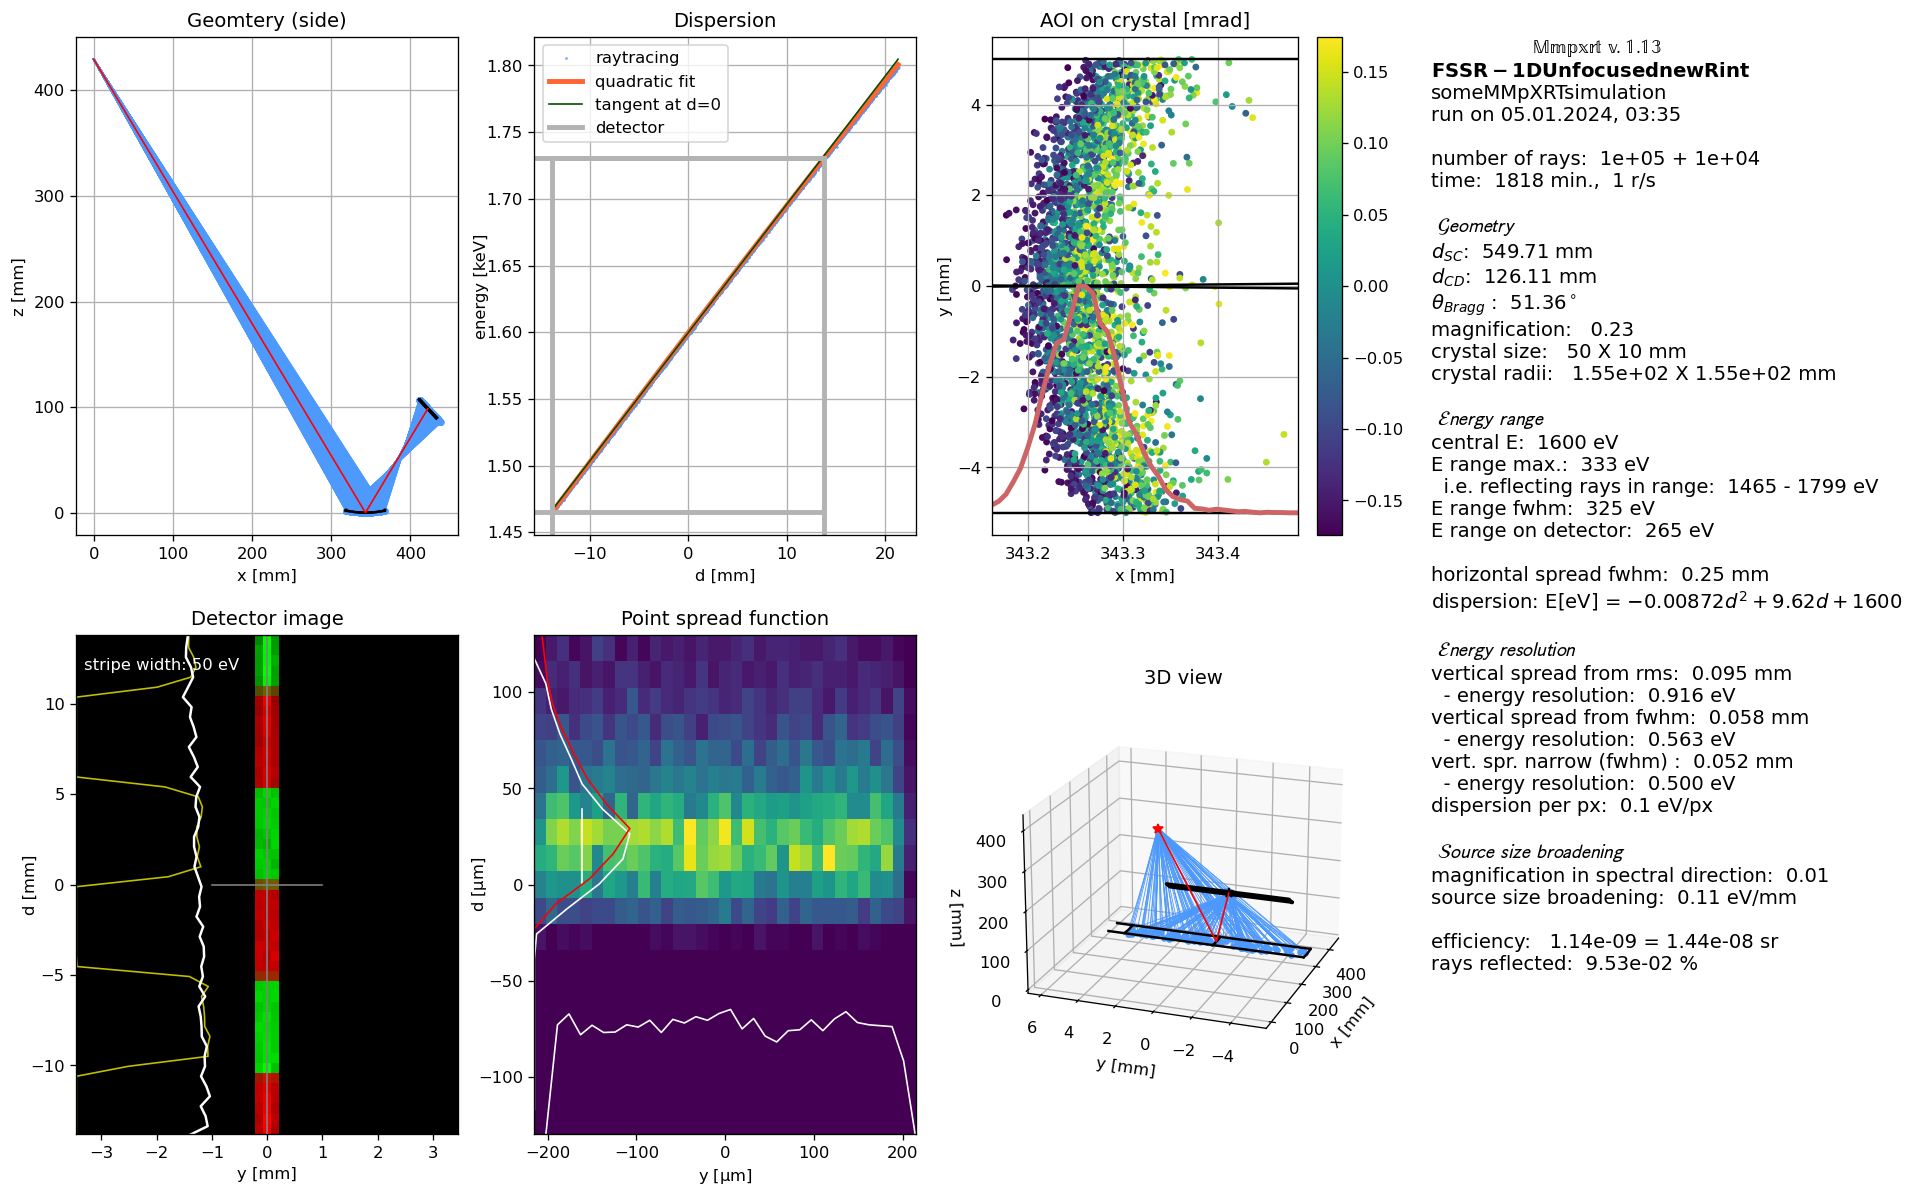
\includegraphics[width=1.15\textwidth, angle=90]{Data_Analysis/mmpxrt_FSSR_new_values.png}
	\caption{Results of \textit{mmpxrt} simulation of the FSSR with an integrated reflectivity of \SI{2.752}{\micro\radian} and a rocking curve width of \SI{349}{\micro\radian}, as derived by Artem's simulation.}
	\label{fig: FSSR new mmpxrt}
\end{figure}

\chapter{Uncertainty Analysis}
\label{chapter: uncertainty analysis}

In this chapter, the error calculations for the quantitative results presented in chapter \ref{chapter: results and discussion} are elaborated on. As section \ref{section: qualitative performance} contains solely qualitative results, only the results of the remaining sections, namely \ref{section: spectrometer characterization} and \ref{section: setup validation}, will be addressed. 

Every error calculation begins with the statistical error, which consists of camera background noise and Poisson noise. I compute the background noise by first getting the standard deviation of the signals of every pixel in the area of the TIFF image from which the background is extracted, e.g. the middle region in fig. \ref{fig: analysis overview}. In the case of the SUCC and DUCC, this standard deviation is then divided by the number of pixel rows $N_{rows}$ that is used for the horizontal lineout of the source spectrum to account for the averaging. For the FSSR, the final background noise corresponds to standard deviation times $\sqrt{N_{rows}}$, since the lineout is formed with summing.

The Poisson noise calculation begins with the raw spectrum extracted by the first part of \textit{AXAWOTLS}, i.e. the counts for each photon energy. As the Poisson noise accounts for the full counts on the ccd chip, for the DUCC and SUCC I multiply $N_{rows}$ onto the raw spectrum counts to approximately undo the averaging of the lineout. The FSSR spectrum is left the same. I then apply equation \ref{eq: detector correction} to get the number of photons incident on the ccd chip. The square root of this number yields the Poisson noise in photons. Inserting this result in the inverse of equation \ref{eq: detector correction} gives the counts noise, which for the DUCC and SUCC is divided by $N_{rows}$ to reinstate the lineout averaging. The sum of the Poisson noise and camera background noise gives the statistical error in counts. As the rest of the spectrum processing steps consist of linear calculations, the statistical error can be propagated just like a standard spectrum, effectively converting it to number of photons per steradian per eV.

For every result, a flat error of 20\% of the mean signal of the peak is imposed on the FSSR, which is added onto the statistical error to account for the poor crystal quality.

\section{Spectral Resolution}

The uncertainty of the FWHM of the fits takes the error of the data points into consideration by nature of the algorithm outlined in section \ref{subsection: spectral resolution}. In this case the only error present on the data is the statistical error. For the cases using the transmission data, the error of both source and transmitted spectra are extended using Gaussian error propagation. The remaining uncertainties of the resolution contributions are determined as follows:
\begin{itemize}
	\item Source broadening: The error of the source size found from the fitting of the knife edge image is carried over to the source broadening through the same path at the source size, since the relations are linear.
	\item Doppler broadening: FLYCHK simulations of Al plasma with an electron temperature of $T_e$ = \SI{1000}{\electronvolt} deliver the base broadening of \SI{0.474}{\electronvolt}. The difference of this value and the Doppler broadening of the He-$\upalpha$ line for $T_e$ = \SI{500}{\electronvolt} corresponds to the error.
	\item Crystal broadening: Gaussian error propagation is applied to equation \ref{eq: crystal broadening}, giving
	\begin{equation}
		s_{crystal} = \frac{1}{\sigma_{crystal}}\sqrt{\text{FWHM}^2\cdot s_{\text{FWHM}}^2 + \sum_{i} \sigma_i^2\cdot s_i^2},
	\end{equation}
	where $s$ represents the uncertainty of each resolution contribution.
\end{itemize}

\section{Ratio of Integrated Reflectivities}

The error on the data points is a combination of the statistical error and a systematic error in the form of a filter transmission error. The latter is based off a 5\% uncertainty placed on the filter thickness. This relative error is propagated to the filter transmission, which is converted into an absolute error on the counts. The sum of this error and the statistical error builds the uncertainty on the signal. In addition, a systematic error of \SI{5}{\milli\meter} is imposed on the diverging distance and added onto the cumulative error. Through Gaussian error propagation, the error is passed onto the final $R_{int}$ ratio. The same method is applied for the $R_{int}$ of the FSSR computed using the simulated efficiency.

\section{Conversion Efficiency into He-$\upalpha$ Emission Line of Aluminum}

The uncertainty of $CE$ is determined analogously to that of the $R_{int}$ ratio, except that an additional 50\% relative error is assumed for the literature $R_{int}$ values, as estimated from the comparison of the experimental $R_{int}$ ratios with the literature. This uncertainty is incorporated in the same way as with that of the diverging distance $D$. As such, the error of the $CE$ from the simulated efficiency of the FSSR exhibits a smaller relative error than with the original method, since the uncertainties of $D$ and $R_{int}$ do not play a role.
 







\end{document}
